
%(BEGIN_QUESTION)
% Copyright 2010, Tony R. Kuphaldt, released under the Creative Commons Attribution License (v 1.0)
% This means you may do almost anything with this work of mine, so long as you give me proper credit

Anta at denne solenoiddrevne ventilen åpner når operatøren trykker «åpne»-bryteren, men lukker umiddelbart når «åpne»-bryteren slippes i stedet for å {\it holde seg låst} i åpen stilling til «lukk»-bryteren trykkes:

$$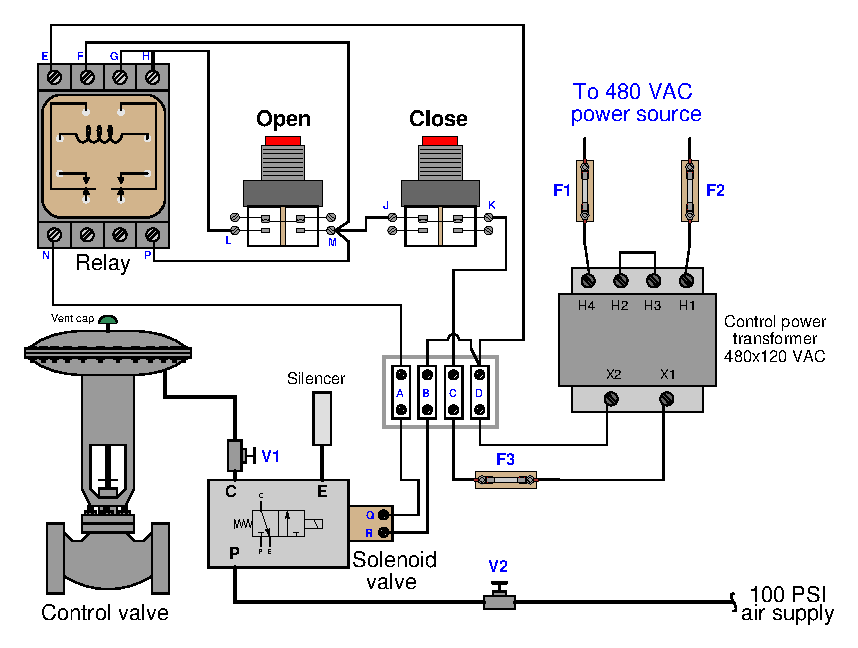
\includegraphics[width=15.5cm]{i00774x01.eps}$$

Du måler 481 volt mellom terminalene {\bf H1} og {\bf H4} på transformatoren, og 118 volt mellom terminalene {\bf M} og {\bf D}, med begge trykknapper upresset.

Vurder sannsynligheten for hver oppgitt feil i dette systemet. Vurder én feil om gangen (dvs. ingen sammenfallende feil), og avgjør om hver feil alene kan forklare {\it alle} målinger og symptomer.

% No blank lines allowed between lines of an \halign structure!
% I use comments (%) instead, so that TeX doesn't choke.

$$\vbox{\offinterlineskip
\halign{\strut
\vrule \quad\hfil # \ \hfil &
\vrule \quad\hfil # \ \hfil &
\vrule \quad\hfil # \ \hfil \vrule \cr
\noalign{\hrule}
%
% First row
{\bf Feil} & {\bf Mulig} & {\bf Umulig} \cr
%
\noalign{\hrule}
%
% Another row
Sikring F3 røket (feilet åpen) &  &  \cr
%
\noalign{\hrule}
%
% Another row
Solenoidespole feilet åpen &  &  \cr
%
\noalign{\hrule}
%
% Another row
«Åpne»-bryterkontakt (L til M) feilet åpen &  &  \cr
%
\noalign{\hrule}
%
% Another row
«Lukk»-bryterkontakt (J til K) feilet åpen &  &  \cr
%
\noalign{\hrule}
%
% Another row
Reléspole feilet åpen &  &  \cr
%
\noalign{\hrule}
%
% Another row
Relékontakt (G til P) feilet åpen &  &  \cr
%
\noalign{\hrule}
%
% Another row
Relékontakt (F til N) feilet åpen &  &  \cr
%
\noalign{\hrule}
%
% Another row
Brudd i leder mellom terminal K og C &  &  \cr
%
\noalign{\hrule}
%
% Another row
Ventil V2 stengt &  &  \cr
%
\noalign{\hrule}
} % End of \halign
}$$ % End of \vbox

Forklar også hvorfor den aller første spenningsmålingen (481 volt mellom H1 og H2) var et bortkastet steg, og angi én mulig feil til som ikke står i tabellen.

Til slutt: angi {\it neste} diagnostiske test eller måling du ville gjort på systemet. Forklar hvordan resultatet/resultatene av testen bidrar til å avklare plassering og/eller type feil.

\underbar{file i00774}
%(END_QUESTION)





%(BEGIN_ANSWER)

% No blank lines allowed between lines of an \halign structure!
% I use comments (%) instead, so that TeX doesn't choke.

$$\vbox{\offinterlineskip
\halign{\strut
\vrule \quad\hfil # \ \hfil &
\vrule \quad\hfil # \ \hfil &
\vrule \quad\hfil # \ \hfil \vrule \cr
\noalign{\hrule}
%
% First row
{\bf Feil} & {\bf Mulig} & {\bf Umulig} \cr
%
\noalign{\hrule}
%
% Another row
Sikring F3 røket (feilet åpen) &  & $\surd$ \cr
%
\noalign{\hrule}
%
% Another row
Solenoidespole feilet åpen &  & $\surd$ \cr
%
\noalign{\hrule}
%
% Another row
«Åpne»-bryterkontakt (L til M) feilet åpen &  & $\surd$ \cr
%
\noalign{\hrule}
%
% Another row
«Lukk»-bryterkontakt (J til K) feilet åpen &  & $\surd$ \cr
%
\noalign{\hrule}
%
% Another row
Reléspole feilet åpen &  & $\surd$ \cr
%
\noalign{\hrule}
%
% Another row
Relékontakt (G til P) feilet åpen & $\surd$ &  \cr
%
\noalign{\hrule}
%
% Another row
Relékontakt (F til N) feilet åpen &  & $\surd$ \cr
%
\noalign{\hrule}
%
% Another row
Brudd i leder mellom terminal K og C &  & $\surd$ \cr
%
\noalign{\hrule}
%
% Another row
Ventil V2 stengt &  & $\surd$ \cr
%
\noalign{\hrule}
} % End of \halign
}$$ % End of \vbox

En god «neste test» er spenningsmåling mellom {\bf P} og {\bf D}, for å se om AC-forsyning faktisk finnes på den reléterminalen (som den skal). En annen god «neste test» er å midlertidig koble terminalene {\bf G} og {\bf P} med en jumper og se om det får ventilen til å bevege seg.

%(END_ANSWER)





%(BEGIN_NOTES)

Første diagnostiske test var bortkastet fordi vi allerede vet at ventilen responderer når «åpne»-trykknappen trykkes. Uten AC-forsyning på transformatoren ville ingenting respondert.

\vskip 10pt

\noindent
Mulige feil som ikke står i tabellen inkluderer:

\begin{itemize}
\item{} Brudd i leder mellom terminal P og M
\item{} Brudd i leder mellom terminal G og H
\end{itemize}

\vskip 10pt

At systemet ikke holder seg innkoblet («latcher») forteller oss at problemet må ligge i reléets latch-del av kretsen. Kontakten som skal «self-holde» den elektriske lukningen av «åpne»-trykknappen gjør på en eller annen måte ikke jobben sin.

\vskip 20pt \vbox{\hrule \hbox{\strut \vrule{} {\bf Virtuell feilsøking} \vrule} \hrule}

Denne oppgaven egner seg godt som «Virtuell feilsøking»-øvelse. Når diagrammet presenteres for studentene, velger du først en bestemt feil i systemet. Deretter presenterer du ett eller flere symptomer på feilen (noe en operatør/bruker ville merket). Studentene foreslår ulike diagnostiske tester for å finne natur og plassering av feilen, som om de var teknikere i felt. Din oppgave er å oppgi hva resultatene av de foreslåtte testene ville vært, og dokumentere resultatene synlig for alle.

Under og etter øvelsen er det nyttig å stille oppfølgingsspørsmål som:

\begin{itemize}
\item{} Hva forteller resultatet av den siste diagnostiske testen om feilen?
\item{} Anta at resultatet av den siste testen var annerledes. Hva ville det i så fall fortalt om feilen?
\item{} Er den siste diagnostiske testen den beste vi kunne gjort?
\item{} Hva ville vært den ideelle testrekkefølgen for å finne feilen med færrest mulig trinn?
\end{itemize}

%INDEX% Feilsøkingsrepetisjon: elektriske kretser

%(END_NOTES)


